\task{Без пробуксовки}
\begin{itemize}

\itA Машина ездит по окружности вокруг точки, где пересекаются линии, перпендикулярные переднему и заднему колёсам, проходящие через их центр. Эти линии вместе с отрезком между колёсами машины образуют прямоугольный треугольник (см. рисунок), один из углов которого~— 60 градусов, а один из катетов~— \SI{5}{\text{м}}.

Тогда $R = 5 \sqrt{3}$ (отношения сторон прямоугольного треугольника с углом $60^\circ$~— известные величины).

\begin{center}
	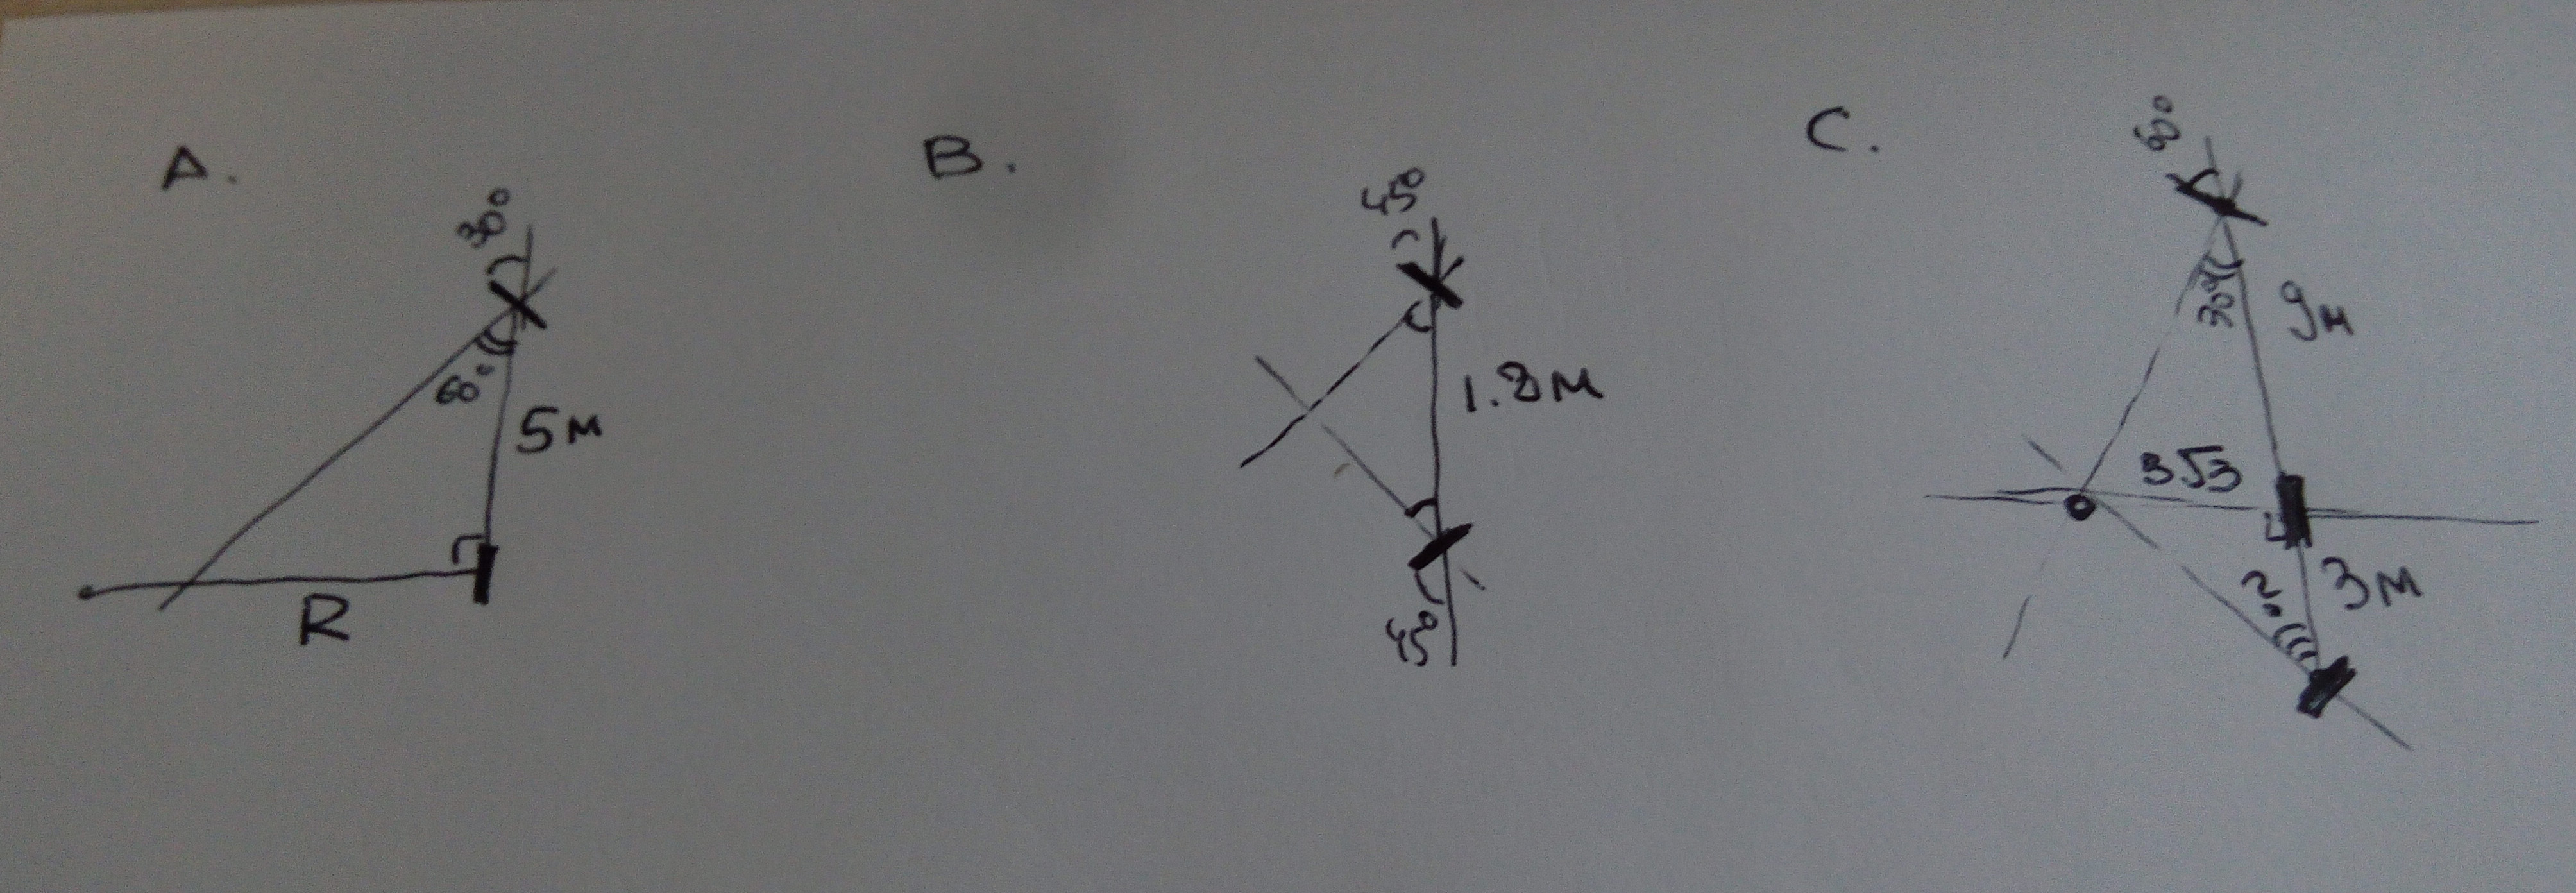
\includegraphics[natwidth=4016,natheight=1392,width=6cm]{figures/2018-cars-no-buks}
\end{center}

\itB Теперь нас интересует высота прямоугольного равнобедренного треугольника с основанием \SI{1.8}{\text{м}}. Она равна \SI{0.9}{\text{м}}. То есть, погрузчик ездит вокруг точки, расположенной на \SI{0.9}{\text{м}} левее, чем середина его левого борта.

\itC Аналогично первому пункту данной задачи, найдём расстояние от не поворачивающегося колеса до точки, вокруг которой ездит автобус. Оно равно $\tfrac{9}{\sqrt{3}} = 3\sqrt{3}$: опять же, мы, зная один из катетов прямоугольного треугольника с углом $60^\circ$, ищем другой.

Теперь заметим, что среднее и заднее колёса, а также точка, вокруг ездит автобус, образуют прямоугольный треугольник с катетами $3$ и $3\sqrt{3}$ метра. Значит, его углы~— 30 и 60 градусов. Отсюда заднее колесо нужно повернуть на 30 градусов.
\end{itemize}